% !TeX root = ../report.tex
% !TeX spellcheck = en-US
% !TeX encoding = UTF-8
\chapter{CONTROLLER DESIGN}\label{chap:controller design}


\section{CRAWLER}
% Describe the current working of the crawler Use diagram and crawler pictures

% Describe the choices that we need to make

% Strategy

% Peripherals

\section{STRATEGY DECISION}\label{sec:strategy decision}
%describe the decision matrix with uncertainties
\import{resources/}{strategy_decision_matrix}

%plot and motivate the choice

\section{PERIPHERALS}\label{sec:peripherals}

\subsection{COMMUNICATION}\label{sec:communication}

\subsubsection{WIRELESS}\label{sec:wireless}

\subsubsection{UMBILICAL}\label{sec:umbilical}


\subsection{LOCALIZATION}\label{sec:localization}

\subsubsection{IMU SENSOR}\label{sec:imu sensor}

\subsubsection{DEPTH SENSOR}\label{sec:depth sensor}
% pressure sensor environment

\subsubsection{SATELLITE DRONES}\label{sec:satalite drones}

% Use GIB text and image compare with kleunen echoes from the deep

\subsection{PROPULSION SENSORS}\label{sec:propulsion sensors}
% torque measurement with the use of a current sensor
% rotational measurement

\subsection{PRODUCTION SENSORS}\lable{sec:production sensors}
% Pressure sensor
% flow sensor

\section{KALMAN FILTER DESIGN}

In Chapter~\ref{chap:cpp} it became evident that an accurate estimation of a crawlers position and heading is needed
such that it can perform its tasks using \gls{acr-CPP} algorithms. Because it is not possible to use \gls{acr-GPS} in an
underwater environment, due to the dampening of electric and magnetic fields in water, which was described in
Section~\ref{sec:em}, an alternative localization method had to be found. Chapter~\ref{chap:coverageunderuncertainty}
describes \gls{gls-Kalman-filter} as the industry de-facto. Position estimation for the control will therefore be
performed with this algorithm.

A design for an \gls{gls-Kalman-filter} is proposed, using a common array of sensors, such as: \gls{gls-accelerometer},
\gls{gls-gyroscope}, \gls{gls-magnetometer} and a \gls{gls-pressure-sensor}. The workings for each of these are
discussed Section~\ref{chap:sensors} and the component selection was made in Section~\ref{sec:strategy decision}. The
crawler is actuated by, changing the rotational speed of the individual \gls{gls-Archimedes-screw}s.

Where the speed of an  \gls{gls-Archimedes-screw} driven crawler is a direct function of the pitch of its vanes. But
this only applies if there is no horizontal soil failure under the screws. Such a phenomena is called slip. It consist
of a period in time where the screws turn, but generate no forwarding force. Leading to an inaccurate estimation for the
new predicted state. Due to the geometry of an \gls{gls-Archimedes-screw}, this slip coexist with an bulldozer effect
created by the vanes acting as a shovel in the soil. This will lead to an increase in torque. It is proposed that by
measuring the required torque of the drive train, a prediction can be made how much slip has occurred, leading to a
better estimation of the future state-vector \gls{sym-x_kt+1}. This behavior and the mathematical model will be
discussed in more detail in Section~\ref{sec:motion model}. Figure~\ref{fig:kalman process} shows the interaction and
connectivity of the various components that server as the input and output of the proposed filter.

Since the physical processes for movement of a crawler are non-linear and the ``basic'' \gls{gls-Kalman-filter},
described in Section~\ref{sec:basic Kalman filter} is limited to linear assumptions, the proposed
\gls{gls-Kalman-filter} is of the Unscented variant. The \gls[first]{acr-UKF} uses a deterministic sampling technique
known as \gls[first]{acr-UT}. This technique picks a minimal set of sample points, also known as sigma points, around
the mean. The sigma points are then propagated through the non-linear function, from which a new mean and covariance
estimate are then formed.

\begin{RoyalFigure}[!htb, label=fig:kalman process]{PROPOSED KALMAN FILTER}
	\begin{center}
		\begin{tikzpicture}[auto, node distance=2cm,>=latex', align=center, inner sep=5mm, thick,scale=0.8, everynode/.style={scale=0.6}]
		\node[block] (controller) {Controller};
		\node[block, right of=controller, xshift=7.5cm] (actuator) {Actuator};
		\node[block, right of=actuator, xshift=1cm] (process) {Process};
		\node[block, below of=actuator] (current) {Current};
		\node[block, below of=current] (gyro) {Gyroscope};
		\node[block, below of=gyro] (acc) {Accelerometer};
		\node[block, below of=acc] (mag) {Magnetometer};
		\node[block, below of=mag](press) {Pressure \\ sensor};
		\node[block, left of=current, xshift=-3cm] (slip predict) {Slip \\ Predict};
		\node[block, left of=slip predict, xshift=-1cm, fill=RoyalLightGrey] (soil param) {Soil \\ Parameters};
		\node[block, below of=soil param, fill=RoyalLightGrey] (geo param) {Geometry \\ Parameters};
		\node[block, below of=slip predict, yshift=-6cm] (kalman) {Unscented \\ Kalman \\ filter};
		\node[output, right of=process](output) {};
		\node[blockdashedwhite, label=below:{\large \textbf{Measurement}},fit={(current) (acc) (mag) (press)} ] (measurement) {};
		\node[blockdashedwhite, label=below:{\large \textbf{microcontroller}},fit={(controller) (kalman) (slip predict)} ] (microcontroller) {};

		\draw[-latex] (controller) -- (actuator) node[midway,above,yshift=-5mm] {\gls{sym-u}};
		\draw[-latex] (actuator) -- (process) node[midway,above,yshift=-5mm] {$ \tau $, $ \omega $ };
		\draw (actuator.east) -| ($(current.east)+(0.5,0)$);
		\draw[-latex] ($(current.east)+(0.5,0)$) -- (current.east);
		\draw[-latex] (process.east) -- (output);
		\draw[-latex] (current.west) -- (slip predict.east)  node[midway,above,yshift=-5mm] { $I$ };
		\draw[-latex] (soil param.east) -- (slip predict.west);
		\draw (geo param.east) -| ($(slip predict.west)-(0.5,0)$);
		\draw[-latex] (slip predict.south) -- (kalman.north) node[midway,above,xshift=-3mm] { $u_k^{\prime}$ };
		\draw[-latex] (kalman.west) -| (controller.south) node[midway,above,yshift=-5mm,xshift=1.5cm] { $\gls{sym-x_k}$} ;
		\draw[-latex] (press.west) -- (kalman.east)  node[midway,above,yshift=5mm] { $\gls{sym-y_k}$ };
		\draw (gyro.west) -| ($(kalman.east)+(1,0)$);
		\draw (acc.west) -| ($(kalman.east)+(1,0)$);
		\draw (mag.west) -| ($(kalman.east)+(1,0)$);
		\draw[-latex] ($(process.east)+(0.5,0)$) |- (gyro.east);
		\draw[-latex] ($(process.east)+(0.5,0)$) |- (acc.east);
		\draw[-latex] ($(process.east)+(0.5,0)$) |- (mag.east);
		\draw[-latex] ($(process.east)+(0.5,0)$) |- (press.east);
		\node[right of=process, xshift=1.5mm,yshift=0.5mm] (x) {$x$};
		\end{tikzpicture}
	\end{center}
\end{RoyalFigure}

\subsection{STATE REPRESENTATION}\label{sec:state representation}

\citet{bahr_cooperative_2009} states that, the most generic case of a vehicle operating in 3D Euler-space, such as a
crawler, consist of a vector of variables comprised of a vehicle's pose and orientation. The pose is its position in a
(global) reference frame \( \left[\gls{sym-x} ~\gls{sym-y} ~\gls{sym-z}\right]^T \). While  its orientation is given in
Euler angles \( \left[\gls{sym-phi_c} ~\gls{sym-psi_c} ~\gls{sym-theta_c}\right]^T \). The pose vector at time
\gls{sym-t} is then \( \gls{sym-x_k} = \left[\gls{sym-x} ~\gls{sym-y} ~\gls{sym-z} ~\gls{sym-phi_c} ~\gls{sym-psi_c}
\gls{sym-theta_c}\right]^T \), which will be denoted as  \gls{sym-x_k} for the remainder of this paper. Beside the pose,
the state vector can also contain the first and second derivatives of the pose vector.

\begin{RoyalFigure}[!htb, label=fig:staterepentation]{STATE REPRESENTATION}
	\begin{center}
		\resizebox{0.6\textwidth}{!}{
			\begin{tikzpicture}
			\node[anchor=south west,inner sep=0] (image) at (0,0) {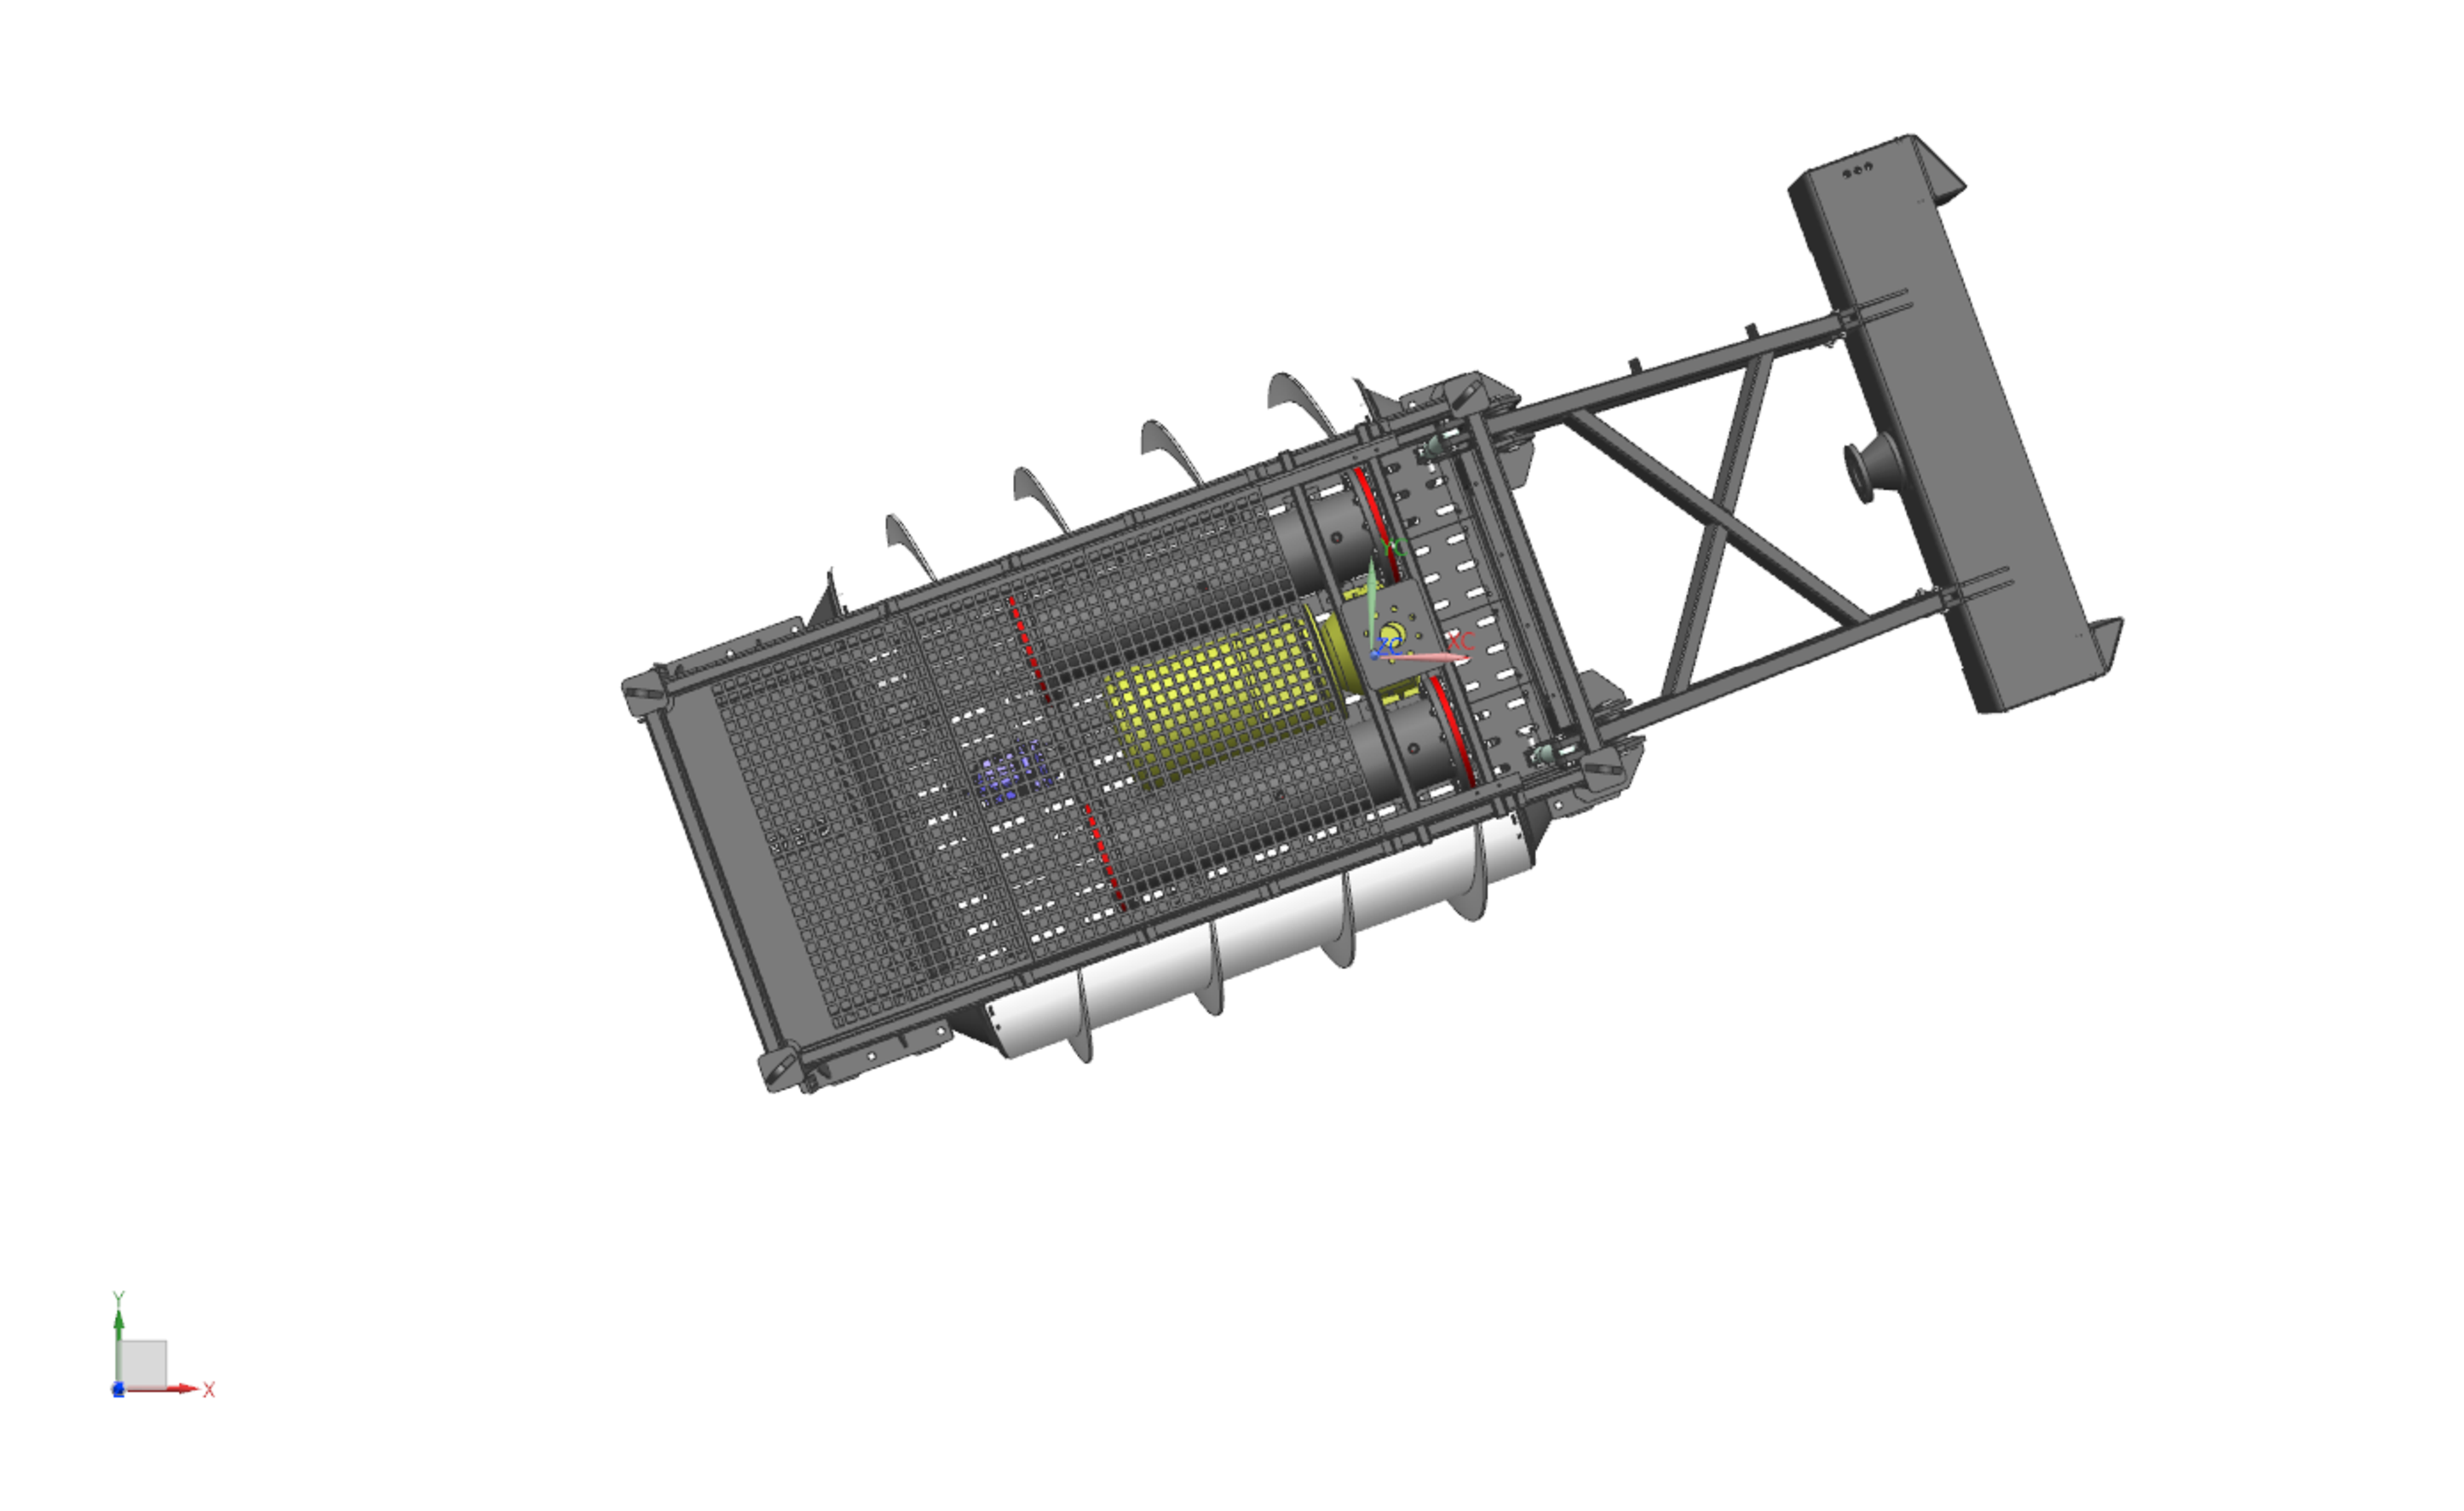
\includegraphics[width=.9\textwidth, trim=2 2 2 2,clip]{dredgebottop.pdf}};
			\node[draw, line width=0.75mm, inner sep=0, circle, minimum size=0.75cm,align=center] (xyz) at (0.6,0.6) {\\ {\huge z}};
			\node[anchor=south west,inner sep=0] (y) at ([shift=(90:8cm)]xyz.center) {{\huge $ y $}};
			\node[anchor=south west,inner sep=0] (x) at ([shift=(00:8cm)]xyz.center) {{\huge $ x $}};
			\node[anchor=south west,inner sep=0] (v_xyz) at (7.9,4.8) {};
			\node[anchor=south west,inner sep=0] (v_xyz_text) at (8,4.2) {$ z^V $};
			\node[anchor=south west,inner sep=0] (v_y) at (7.9,8) {};
			\node[anchor=south west,inner sep=0] (v_x) at (12,4.8) {};
			\node[anchor=south west,inner sep=0] (heading) at ([shift=(22.5:5cm)]v_xyz) {$ x^V $};
			\node[anchor=south west, inner sep=0] (perp_heading) at ([shift=(112.5:3cm)]v_xyz) {$ y^V $};

			\node[anchor=south west,inner sep=0] (vec) at (3,1.5) { $ \gls{sym-x_k} =\left[\gls{sym-x},\gls{sym-y},\gls{sym-z}\right] $ };

			\draw[-latex, line width=0.75mm] (xyz.center) to (x);
			\draw[-latex, line width=0.75mm] (xyz.center) to (y);
			\draw[-latex,red, line width=0.5mm] (xyz.center) to (v_xyz);
			\draw[-latex,green, line width=0.5mm] (v_xyz.center) to (heading);
			\draw[-latex,green, line width=0.5mm] (v_xyz.center) to (perp_heading);
			\draw[dashed, line width=0.25mm] (v_xyz.center) to (v_y.center);
			\draw[dashed, line width=0.25mm] (v_xyz.center) to (v_x.center);

			\draw[latex-latex, line width=0.25mm] ([xshift=2cm]v_xyz.center) arc (0:22.25:2cm) node [right,pos=0.5] {$ \gls{sym-psi_c} $};
			\draw[latex-latex, line width=0.25mm,rotate=22.5] ([xshift=-1cm, yshift=-0.5cm]heading) arc (-120:150:0.20cm and 0.55cm) node [above,pos=0.85] {$ \gls{sym-phi_c} $};
			\draw[latex-latex, line width=0.25mm,rotate=112.5] ([xshift=-1cm, yshift=-0.3cm]perp_heading) arc (-120:150:0.2cm and 0.55cm) node [above,pos=0.65] {\gls{sym-theta_b}};

			\end{tikzpicture}}
	\end{center}
	\caption{State representation}\label{fig:staterepentation}
\end{RoyalFigure}

\subsubsection{2D OR 3D}

\citet{bahr_cooperative_2009} proposes the following simplification; They state that all submersible vehicles are
outfitted with a pressure sensor which allows them to determine their absolute depth with high accuracy and a high
update rate. As a result all underwater navigation systems are only used to resolve the 2D position and all underwater
vehicle related localization problems are stated in 2D. Which allows for a simplified state vector \( \gls{sym-x_k} =
\left[\gls{sym-x} ~\gls{sym-y} ~\gls{sym-phi_c} ~\gls{sym-psi_c} ~\gls{sym-theta_c}\right]^T \).

This simplification does not hold for crawlers or \gls{acr-AUV} that change in depth in any other direction then
collinear with the earths gravitational axis. Since this crawler moves over irregular terrain, any pitch or roll will
result in a gravitational force that also consist of components along the x-axis and / or y-axis. Which would then be
interpreted as movements in the 2D x-y space. This coupled with an unreliable pressure-sensor reading due to
disturbance of sediment from the sea bed during dredging operations, as described in Section~\ref{sec:pressure sensor},
means the the state representation should be in 3D Euler space, as is shown in figure~\ref{fig:staterepentation}.

\subsubsection{\gls{gls-quaternion}S}

Because the \gls{acr-UKF} is run on a embedded device, with limited resources, all rotational translations are
calculated with the help of \gls{gls-quaternion}s. Which make use of the same concept as complex numbers, except of
using one imaginary axis, there are three. Just as complex numbers are very useful in describing a rotation in a
two-dimensional plane, \gls{gls-quaternion}s are highly efficient in a three-dimensional space. They are also immune to
\gls{gls-gimbal-lock}ing. The exact workings are outside of the scope of this thesis, but for those readers which are
interested, a good explanation is given by \citet{3blue1brown_\gls{gls-quaternion}s_2018} and can be found
at~\url{www.youtube.com/watch?v=d4EgbgTm0Bg}. A \gls{gls-quaternion}s is represented as a single column matrix with four
rows, consisting  of a magnitude and three components for the axes \(\gls{sym-q} = \left[\gls{sym-q_s} ~\gls{sym-q_x}
~\gls{sym-q_y}  ~\gls{sym-q_z} \right]^T \), Where the \gls{sym-q_s} is used to normalize the \gls{gls-quaternion}, this
keeps the error from accumulating. It is important to note that \gls{gls-quaternion}s are \gls{gls-non-commutative},
thus the order in which they are applied matters to the outcome of the rotation.


\section{CONTROLLER}\label{sec:controller}

\subsection{THE WORLD}

\subsection{A VESSEL}

\subsection{THE CAPTAIN}

\subsection{THE NAVIGATOR}


\subsection{A BOATSWAIN}
The boatswain is responsible for execution of the different tasks. A crawler has four states of operation, namely:
normal travel, dredging coverage travel, stationary dredging and standstill. These, and their transitions are depicted
in diagram \ref{fig:stateoperating}. These state dictate the maximum travel speed \gls{sym-x_k}. During normal travel, a
crawler moves from a start location to its goal, its traveling speed limited by the  maximum allowable power
delivered to the propulsion system.

\begin{RoyalFigure}[!htb, label=fig:stateoperating]{STATE OPERATIONS}
	\resizebox{9cm}{!}{
		\begin{tikzpicture}[->,>=stealth',shorten >=1pt,auto,node distance=3.5cm,
		semithick, every state/.style={minimum size=3cm, align=center}]

		\node[initial,state,fill=tudelft-orange!10] (standstill) {Standstill};
		\node[state,fill=RoyalLightGrey] (coverage) [right of=standstill, yshift=3cm, xshift=2cm] {Coverage dredging};
		\node[state,fill=RoyalLightGrey] (travel) [below of=coverage, xshift=-2cm, yshift=-2cm] {Travel};
		\node[state,fill=RoyalLightGrey] (localized) [left of=travel, yshift=-2cm, xshift=-2cm] {Localized dredging};
		\node (exit) [left of=standstill, xshift=20mm,yshift=20mm]	{exit};

		\path (standstill) edge [bend right] (travel);
		\path (travel) edge [bend right] (standstill);

		\path (localized) edge [bend right] (travel);
		\path (standstill) edge [bend right] (localized);
		\path (localized) edge [bend right] (standstill);

		\path (standstill) edge [bend right=10] (coverage);
		\path (coverage) edge [bend right=30] (standstill);

		\path (travel) edge [bend right] (coverage);
		\path (coverage) edge [bend right=10] (travel);

		\path (standstill) edge (exit);
		\end{tikzpicture}}
\end{RoyalFigure}

\subsubsection{COVERAGE DREDGING}

\subsubsection{TRAVEL}

\subsubsection{LOCALIZED DREDGING}
